\documentclass[a4paper,ngerman,12pt]{scrartcl}

\usepackage[utf8]{inputenc}
%\usepackage[ansinew]{inputenc}

\usepackage[ngerman]{babel}

\usepackage{amsmath,amsthm,amssymb,stmaryrd,color,graphicx}
\usepackage{setspace}
\usepackage{bussproofs}
\usepackage{array}
\usepackage{comment}

\usepackage{enumitem}

\usepackage[protrusion=true,expansion=true]{microtype}

\usepackage{lmodern}

\usepackage{hyperref}
\usepackage{cleveref}

\newcommand{\RR}{\mathbb{R}}
\newcommand{\CC}{\mathbb{C}}
\newcommand{\ZZ}{\mathbb{Z}}
\newcommand{\NN}{\mathbb{N}}
\newcommand{\QQ}{\mathbb{Q}}

\setlength\parskip{\medskipamount}
\setlength\parindent{0pt}

\theoremstyle{definition}
\newtheorem{defn}{Definition}[]
\newtheorem{axiom}[defn]{Axiom}
\newtheorem{bsp}[defn]{Beispiel}

\theoremstyle{plain}
\newtheorem{prop}[defn]{Proposition}
\newtheorem{motto}[defn]{Motto}
\newtheorem{wunder}[defn]{Wunder}
\newtheorem{ueberlegung}[defn]{Überlegung}
\newtheorem{lemma}[defn]{Lemma}
\newtheorem{kor}[defn]{Korollar}
\newtheorem{hilfsaussage}[defn]{Hilfsaussage}
\newtheorem{satz}[defn]{Satz}

\theoremstyle{remark}
\newtheorem{bem}[defn]{Bemerkung}
\newtheorem{aufg}[defn]{Aufgabe}

\newlength{\aufgabenskip}
\setlength{\aufgabenskip}{1.4em}
\newcounter{aufgabennummer}
\newenvironment{aufgabe}[1]{
  \addtocounter{aufgabennummer}{1}
  \textbf{Aufgabe \theaufgabennummer.} \emph{#1} \par
}{\vspace{\aufgabenskip}}

\clubpenalty=10000
\widowpenalty=10000
\displaywidowpenalty=10000

\setlength\unitlength{1cm}

\usepackage{tikz}
\def\mkPascal#1{
  \begin{tikzpicture}
    \def\dx{20pt}
    \def\dy{30pt}
    \newcounter{i}
    \stepcounter{i}
    \node (\arabic{i}) at (0,0) {1};
    \foreach [count=\i] \x in {2,...,#1}{
      \pgfmathsetmacro{\lox}{\x-1}%
      \pgfmathsetmacro{\loxt}{\x-3}%
      \foreach [count=\j] \xx in {-\lox,-\loxt,...,\lox}{
        \pgfmathsetmacro{\jj}{\j-1}%
        \stepcounter{i}
        \pgfmathsetmacro{\lbl}{\lox!/(\jj!*(\lox-\jj)!)}
        \node  (\arabic{i}) at (\xx*\dx, -\lox*\dy) {\pgfmathint{\lbl}\pgfmathresult};
      }
    }
    \newcounter{z}
    \newcounter{xn}
    \newcounter{xnn}
    \pgfmathsetmacro{\maxx}{#1 - 1}
    \foreach \x in {1,...,\maxx}{
      \foreach \xx in {1,...,\x}{
        \stepcounter{z}
        \setcounter{xn}{\arabic{z}}
        \addtocounter{xn}{\x}
        \setcounter{xnn}{\arabic{xn}}
        \stepcounter{xnn}
          \draw [->] (\arabic{z}) -- (\arabic{xn});
          \draw [->] (\arabic{z}) -- (\arabic{xnn});
      }
    }
  \end{tikzpicture}
}

\RequirePackage{geometry}
\geometry{textwidth=16.0cm,textheight=24.5cm,footskip=1.5cm}

\begin{document}

\begin{picture}(0,0)
  \put(0,-0.5){%
    
\includegraphics[scale=0.1]{logo-ifm}
  }
  \put(14.0,-3.5){%
    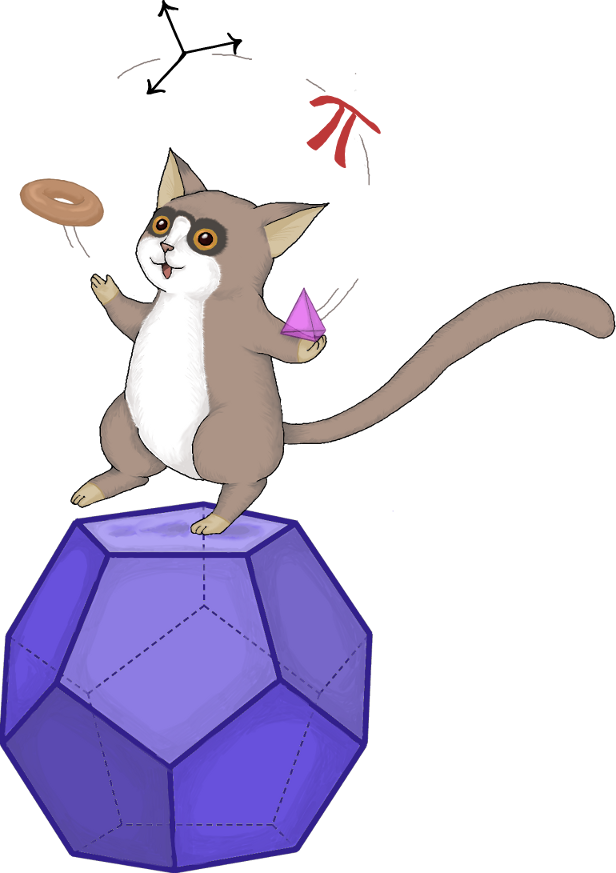
\includegraphics[scale=0.17]{cover}
  }
\end{picture} 

\vspace{6em}

\begin{center}\Large{Dritter Korrespondenzbrief}\end{center}

\section*{Fraktale Dimensionen}

Einleitung!


\section{Die Kochsche Schneeflocke}

Ersten zwei Schritte einer Konstruktion eines Musters:

\begin{center}
	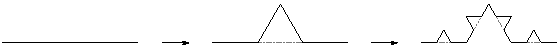
\includegraphics[width=.9\textwidth]{Bilder/Schneeflocke-Konstruktion1.pdf}
\end{center}

Wie du siehst, beginnt alles mit einer einfachen Strecke. Diese Strecke teilen wir in drei gleich lange Teile. Dann entfernen wir das mittlere Stück und ersetzen es durch die zwei anderen Seiten eines gleichseitigen Dreiecks. Dadurch erhalten wir eine geometrische Figur, die aus vier Strecken besteht. Für den zweiten Schritt machen wir nun mit jeder dieser vier Strecken das gleiche wie wir es mit der ersten Strecke getan haben.

Kannst du den dritten Schritt jetzt selbst zeichnen?

\begin{center}
	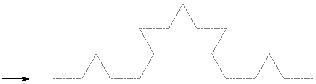
\includegraphics[width=.7\textwidth]{Bilder/Schneeflocke-Konstruktion2.pdf}
\end{center}

Wenn du möchtest kannst du auch noch einen vierten Schritt zeichnen. Schaffst du sogar einen fünften? Ziemlich bald wird es vermutlich schwierig noch weitere Schritte zu machen - einfach weil die Strecken so kurz werden, dass wir sie nicht mehr vernünftig teilen können. Aber zumindest vorstellen können wir uns doch, dass wir mit diesem Verfahren immer weiter machen - einen siebten Schritt, einen achten Schritt, usw. 

\begin{center}
	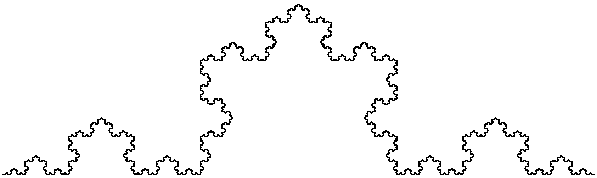
\includegraphics[width=.5\textwidth]{Bilder/Schneeflocke-Konstruktion3.pdf}
\end{center}

Tatsächlich wollen wir sogar \glqq unendlich viele\grqq{} Schritte machen und uns fragen, was für ein geometrisches Objekt wir dadurch erhalten. Dieses Objekt können wir natürlich nicht mehr zeichnen, aber wir können uns trotzdem überlegen, was für Eigenschaften dieses Objekt haben muss. Und genau das wollen wir in diesem Brief tun. 

Als erstes wollen wir uns einmal überlegen, wie lang die Linie wohl sein muss, aus der unser Objekt \glqq nach unendlich vielen Schritten\grqq{} besteht. Da wir es nicht zeichnen können, können wir natürlich nicht einfach nachmessen. Statt dessen wollen wir uns überlegen, was in einem einzelnen Schritt mit der Länge der Linie geschieht.

Dazu wollen wir annehmen, dass die Strecke ganz zu Beginn die Länge $l$ hat. Wie ist dann die Länge der Linie nach dem ersten Schritt? Nun, zuerst wir haben die Strecke in drei gleich lange Strecken geteilt und die mittlere davon entfernt - bleibt also noch eine Länge von $\frac{2}{3}l$. Dann haben wir in der Mitte zwei Seiten eines gleichseitigen Dreiecks gezeichnet, wobei jede der beiden Seiten so lang ist, wie die beiden Strecken. Also hat unsere gesamte Linie nach dem zweiten Schritt eine Länge von $\frac{2}{3}l + 2\cdot\frac{1}{3}l = \frac{4}{3}l$. Unsere neue Linie ist also $\frac{4}{3}$-mal so lang wie die ursprüngliche (miss in der Zeichnung doch einmal nach, ob das auch tatsächlich stimmt!).

Was passiert nun im zweiten Schritt? ...



\begin{bem}Wo ist jetzt die Schneeflocke? Beginne mit einem Dreieck:
	\begin{center}
		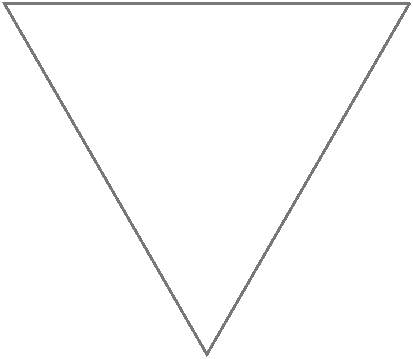
\includegraphics[width=.6\textwidth]{Bilder/Eigene_Schneeflocke.pdf}
	\end{center}	
\end{bem}




\section{Dimensionen}


\begin{defn}
Definition der Fraktalen Dimension\footnote{Tatsächlich gibt es mehrere Möglichkeiten fraktale Dimensionen zu definieren - wir betrachten hier die sogenannte \glqq Ähnlichkeits-Dimension\grqq{}}
\end{defn}

\begin{bem}
Logarithmus mit Taschenrechner berechnen
\end{bem}

\section{Mehr Fraktale}

Sierpinski-Dreieck (Erinnerung an Pascalsches Dreieck!)

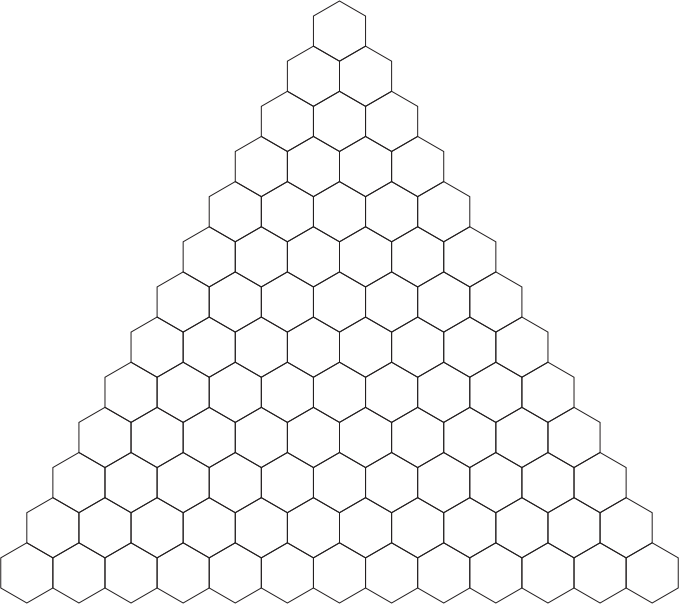
\includegraphics{Bilder/pascal-triangle.png}

evtl. Menger-Schwamm

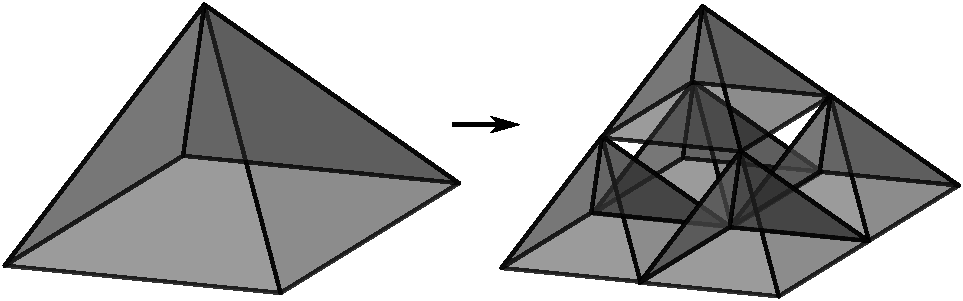
\includegraphics{Bilder/Pyramiden.pdf}

evtl. Drachenkurve (Basteln!)

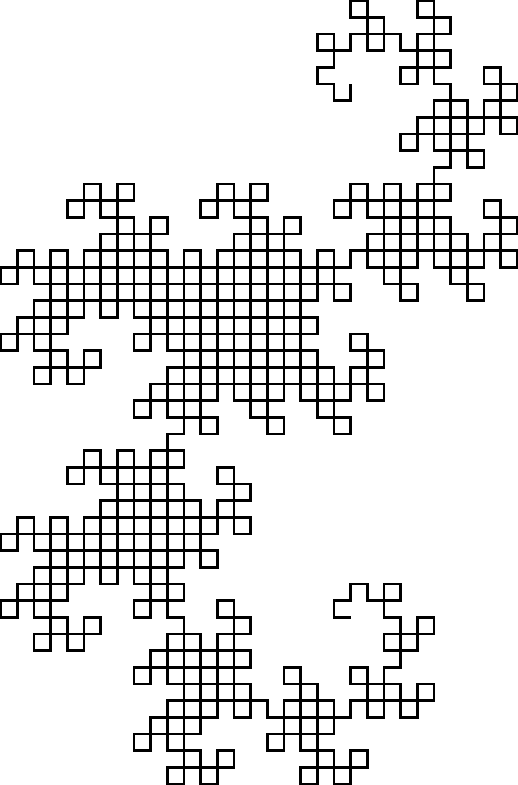
\includegraphics{Bilder/Drachenkurve.pdf}

\section{Fraktale im echten Leben}

Küstenlinie messen?

\end{document}
